\documentclass[11pt]{article}
\usepackage[margin=0.7in]{geometry} 
\usepackage{amsmath,amsthm,amssymb,amsfonts}
\usepackage{enumitem}
\usepackage{dsfont}
\usepackage{soul}
\usepackage{mathtools}
\usepackage[utf8]{inputenc}
\usepackage{multirow}
\usepackage[colorlinks]{hyperref}
\usepackage{cleveref}
\usepackage{bm}
\usepackage{tikz-cd}
\usepackage{adjustbox}
\usepackage[normalem]{ulem}
\usepackage{authblk}
\usepackage{listings}
\usepackage{xcolor}
\usepackage{graphicx}


\renewcommand{\baselinestretch}{1.25}
 
\newtheorem{lemma}{Lemma}
\newtheorem{claim}{\sf Claim}
\newtheorem{defi}{Definition}
\newtheorem{thm}{Theorem}
\newtheorem{cor}{Corollary}
\newtheorem{prop}{Proposition}
\newtheorem{rmk}{\it Remark}
\newtheorem{ex}{Example}
\newtheorem{notation}{Notation}
\newtheorem{algorithm}{Algorithm}
\newtheorem{assumption}{Assumption}
\newtheorem{problem}{Problem}

\DeclareMathOperator*{\argmin}{argmin}
\DeclareMathOperator*{\argmax}{argmax}

\definecolor{codegreen}{rgb}{0,0.6,0}
\definecolor{codegray}{rgb}{0.5,0.5,0.5}
\definecolor{codepurple}{rgb}{0.58,0,0.82}
\definecolor{backcolour}{rgb}{0.95,0.95,0.92}

\lstdefinestyle{mystyle}{
    backgroundcolor=\color{backcolour},   
    commentstyle=\color{codegreen},
    keywordstyle=\color{magenta},
    numberstyle=\tiny\color{codegray},
    stringstyle=\color{codepurple},
    basicstyle=\ttfamily\footnotesize,
    breakatwhitespace=false,         
    breaklines=true,                 
    captionpos=b,                    
    keepspaces=true,                 
    numbers=left,                    
    numbersep=5pt,                  
    showspaces=false,                
    showstringspaces=false,
    showtabs=false,                  
    tabsize=2
}

\lstset{style=mystyle}
  
\begin{document}
 
\title{MAS374 Optimization theory\\ Homework \#3}
\author{20150597 Jeonghwan Lee}
\affil{Department of Mathematical Sciences, KAIST}

\maketitle

I worked on this programming assignment by using Python 3 (version 3.7.7). I utilized PyCharm 2021.1 Community Edition as an integrated development environment (IDE). \\ [10pt]
\indent (a) The next code defines a function \texttt{my\_lstsq(A, y)} which takes $\mathbf{A} \in \mathbb{R}^{m \times n}$ and $\mathbf{y} \in \mathbb{R}^m$ as its input and employs the singular value decomposition of $\mathbf{A}$ to compute and return the optimal solution $\bm{\theta}^* = \mathbf{A}^{\dagger} \mathbf{y} \in \mathbb{R}^n$:

\begin{lstlisting}[language = Python]
import numpy as np

def my_lstsq(A, y):
    m = A.shape[0]
    n = A.shape[1]
    r = np.linalg.matrix_rank(A)
    u, s, vh = np.linalg.svd(A, full_matrices=True)
    pseudo_smat = np.zeros((n, m))
    for i in range(r):
        pseudo_smat[i, i] = 1/s[i]
    pseudo_inv_A = np.dot(np.transpose(vh), np.dot(pseudo_smat, np.transpose(u)))
    theta = np.dot(pseudo_inv_A, y)
    return theta
\end{lstlisting}

\noindent For a simpler implementation of the function \texttt{my\_lstsq(A, y)}, we may use the following code which defines a function \texttt{my\_lstsq\_simpler(A, y)} that uses the Moore-Penrose pseudo-inverse $\mathbf{A}^{\dagger} \in \mathbb{R}^{n \times m}$ directly. Note that the function \texttt{my\_lstsq\_simpler(A, y)} does not use the \textsf{SVD} of $\mathbf{A}$ in the code:

\begin{lstlisting}[language = Python]
import numpy as np

def my_lstsq_simpler(A, y):
    pseudoinv_A = np.linalg.pinv(A)
    theta = np.dot(pseudoinv_A, y)
    return theta
\end{lstlisting}

\noindent It is worth to notice that both the functions \texttt{my\_lstsq(A, y)} and \texttt{my\_lstsq\_simpler(A, y)} requires no full column-rank condition of $\mathbf{A}$; $m \geq n = \textsf{rank}(\mathbf{A})$. So the above codes provide the optimal solution $\bm{\theta}^* = \mathbf{A}^{\dagger} \mathbf{y}$ under the fully general case. \\ [10pt]
\indent (b) Here, we generate $n$ samples $\left\{ \mathbf{x}^{(i)} := \left( x_{1}^{(i)}, x_{2}^{(i)} \right) : i \in [n] \right\}$ from $\textsf{Unif} \left( [-2, 2] \times [-2, 2] \right)$. Note that we are letting $n = 250$ in this problem. We first label these sample points according to the rule
\begin{equation}
    \label{eqn1}
    y_i =
    \begin{cases}
        +1 & \textnormal{if } \left( x_{1}^{(i)} \right)^2 + \left( x_{2}^{(i)} \right)^2 \leq 1; \\
        -1 & \textnormal{otherwise,}
    \end{cases}
\end{equation}
and let $\mathbf{y} := \begin{bmatrix} y_1 & y_2 & \cdots & y_n \end{bmatrix}^{\top} \in \mathbb{R}^n$. The construction of the samples $\left\{ \mathbf{x}^{(i)} := \left( x_{1}^{(i)}, x_{2}^{(i)} \right) : i \in [n] \right\}$ and the label vector $\mathbf{y} \in \mathbb{R}^n$ (here, $n = 250$) can be implemented through the following code:
\begin{lstlisting}[language = Python]
import numpy as np
import random

def label(a, b):     # label a given point in \mathbb{R}^2
    if a**2 + b**2 <= 1:
        return 1
    else:
        return -1

length = 250     # number of samples
first_coordinate_1 = np.dot(4, np.random.rand(length)) - np.dot(2, np.ones(length))       # the first coordinates of 250 samples chosen uniformly at random from [-2, 2] \times [-2, 2]
second_coordinate_1 = np.dot(4, np.random.rand(length)) - np.dot(2, np.ones(length))      # the second coordinates of 250 samples chosen uniformly at random from [-2, 2] \times [-2, 2]
y_1 = np.zeros(length)     # initialize vector of labels for part (b)
num_1 = 0
for i in range(length):
    y_1[i] = label(first_coordinate_1[i], second_coordinate_1[i])     # label the 250 random sample points according to the rule (4)
    if y_1[i] > 0:
        num_1 = num_1 + 1
\end{lstlisting}

\indent Next, we would like to construct our coefficient matrix $\mathbf{A} \in \mathbb{R}^{n \times 6}$ from the samples $\left\{ \mathbf{x}^{(i)} := \left( x_{1}^{(i)}, x_{2}^{(i)} \right) : i \in [n] \right\}$ as follows: for every $i \in [n]$, the $i$-th row vector of $\mathbf{A}$ is given by
\begin{equation*}
    \begin{split}
        \mathbf{A}_{i*} := 
        \begin{bmatrix}
            1 & x_{1}^{(i)} & x_{2}^{(i)} & x_{1}^{(i)} x_{2}^{(i)} & \left( x_{1}^{(i)} \right)^2 & \left( x_{2}^{(i)} \right)^2
        \end{bmatrix}
    \end{split}
\end{equation*}
The construction of the coefficient matrix $\mathbf{A} \in \mathbb{R}^{n \times 6}$ can be implemented through the following code:
\begin{lstlisting}[language = Python]
import numpy as np

def generate_data_matrix(first_coordinate, second_coordinate):     # construct a proper data matrix (2-dimensional array) of shape length \times 6
    input_length = first_coordinate.shape[0]
    data_matrix = np.zeros((length, 6))
    for i in range(input_length):
        data_matrix[i, 0] = 1
        data_matrix[i, 1] = first_coordinate[i]
        data_matrix[i, 2] = second_coordinate[i]
        data_matrix[i, 3] = first_coordinate[i]**2
        data_matrix[i, 4] = first_coordinate[i]*second_coordinate[i]
        data_matrix[i, 5] = second_coordinate[i]**2
    return data_matrix
\end{lstlisting}

\noindent By utilizing the coefficient matrix $\mathbf{A} \in \mathbb{R}^{n \times 6}$ and the label vector $\mathbf{y} \in \mathbb{R}^n$, we can compute the LS solution $\bm{\theta}^* = \mathbf{A}^{\dagger} \mathbf{y} \in \mathbb{R}^6$, which is an optimal solution to the following least-squares problem:
\begin{equation}
    \label{eqn2}
    \min_{\bm{\theta} \in \mathbb{R}^6} \left\| \mathbf{y} - \mathbf{A} \bm{\theta} \right\|_{2}^2.
\end{equation}
This part can be performed by using the function \texttt{my\_lstsq(A, y)}:
\begin{lstlisting}[language = Python]
import numpy as np

A_1 = generate_data_matrix(first_coordinate_1, second_coordinate_1)
theta_1 = my_lstsq(A_1, y_1)  # compute the optimal order-2 polynomial that minimizes (3)
print(theta_1)
\end{lstlisting}

\indent Lastly, we would like to determine how the decision boundary would look like in a quantitative way, and visualize it by using \href{https://matplotlib.org/stable/api/_as_gen/matplotlib.pyplot.html}{matplotlib.pyplot}. To this end, we first introduce how to classify the conic sections by using its discriminant. We consider the conic section $A x^2 + B xy + C y^2 + Dx + Ey + F = 0$. The discriminant of this conic section is defined by $\Delta := B^2 - 4AC$. Then it is well-known that
\begin{enumerate}
    \item if $A = C$ and $B = 0$, then the equation $A x^2 + B xy + C y^2 + Dx + Ey + F = 0$ represents a circle, which is a special case of an ellipse;
    \item if $\Delta < 0$, then the equation $A x^2 + B xy + C y^2 + Dx + Ey + F = 0$ represents an ellipse;
    \item if $\Delta = 0$, then the equation $A x^2 + B xy + C y^2 + Dx + Ey + F = 0$ represents a parabola;
    \item if $\Delta > 0$, then the equation $A x^2 + B xy + C y^2 + Dx + Ey + F = 0$ represents a hyperbola.
\end{enumerate}
See \cite{protter1988calculus} for further details of the classification of conic sections. Utilizing these facts, one can design a function \texttt{conic\_section\_discriminant(A, B, C, D, E, F)} as follows:
\begin{lstlisting}[language = Python]
def conic_section_discriminant(A, B, C, D, E, F):        # discriminate the conic section Ax^2 + Bxy + Cy^2 + Dx + Ey + F = 0
    discriminant = B**2 - 4*A*C
    if A == C and B == 0:
        return "Circle"
    elif discriminant < 0:
        return "Ellipse"
    elif discriminant == 0:
        return "Parabola"
    else:
        return "Hyperbola"
\end{lstlisting}
Upon establishing this function, we are now able to verify the shape of the decision boundary by using the above facts and visualize it by implementing the following code:
\begin{lstlisting}[language = Python]
import numpy as np
import random
import matplotlib as mpl
import matplotlib.pyplot as plt

def axes():
    plt.axhline(0, alpha=.1)
    plt.axvline(0, alpha=.1)

print(conic_section_discriminant(theta_1[3], theta_1[4], theta_1[5], theta_1[1], theta_1[2], theta_1[0]))     # discriminate the conic section formed as the zero set of the optimal order-2 polynomial that minimizes (3) (= the decision boundary)

x = np.linspace(-5, 5, 4000)
y = np.linspace(-5, 5, 4000)
x, y = np.meshgrid(x, y)
axes()
plt.contour(x, y, (theta_1[3]*x**2 + theta_1[4]*x*y + theta_1[5]*y**2 + theta_1[1]*x + theta_1[2]*y + theta_1[0]), [0], colors='k')
plt.show()
\end{lstlisting}

\indent To sum up, the overall code for part (b) can be encapsulated as follows:
\begin{lstlisting}[language = Python]
import numpy as np
import random
import matplotlib as mpl
import matplotlib.pyplot as plt

def axes():
    plt.axhline(0, alpha=.1)
    plt.axvline(0, alpha=.1)

def label(a, b):     # label a given point in \mathbb{R}^2 according to the rule (4)
    if a**2 + b**2 <= 1:
        return 1
    else:
        return -1

def generate_data_matrix(first_coordinate, second_coordinate):      # construct a proper data matrix (2-dimensional array) of shape length \times 6
    input_length = first_coordinate.shape[0]
    data_matrix = np.zeros((length, 6))
    for i in range(input_length):
        data_matrix[i, 0] = 1
        data_matrix[i, 1] = first_coordinate[i]
        data_matrix[i, 2] = second_coordinate[i]
        data_matrix[i, 3] = first_coordinate[i]**2
        data_matrix[i, 4] = first_coordinate[i]*second_coordinate[i]
        data_matrix[i, 5] = second_coordinate[i]**2
    return data_matrix

def conic_section_discriminant(A, B, C, D, E, F):       # discriminate the conic section Ax^2 + Bxy + Cy^2 + Dx + Ey + F = 0
    discriminant = B**2 - 4*A*C
    if A == C and B == 0:
        return "Circle"
    elif discriminant < 0:
        return "Ellipse"
    elif discriminant == 0:
        return "Parabola"
    else:
        return "Hyperbola"

length = 250     # number of samples
first_coordinate_1 = np.dot(4, np.random.rand(length)) - np.dot(2, np.ones(length))       # the first coordinates of 250 samples chosen uniformly at random from [-2, 2] \times [-2, 2]
second_coordinate_1 = np.dot(4, np.random.rand(length)) - np.dot(2, np.ones(length))      # the second coordinates of 250 samples chosen uniformly at random from [-2, 2] \times [-2, 2]
y_1 = np.zeros(length)     # initialize vector of labels for part (b)
num_1 = 0
for i in range(length):
    y_1[i] = label(first_coordinate_1[i], second_coordinate_1[i])     # label the 250 random sample points according to the rule (4)
    if y_1[i] > 0:
        num_1 = num_1 + 1

A_1 = generate_data_matrix(first_coordinate_1, second_coordinate_1)
theta_1 = my_lstsq(A_1, y_1)     # compute the optimal order-2 polynomial that minimizes (3)
print(theta_1)
print(conic_section_discriminant(theta_1[3], theta_1[4], theta_1[5], theta_1[1], theta_1[2], theta_1[0]))     # discriminate the conic section formed as the zero set of the optimal order-2 polynomial that minimizes (3) (= the decision boundary)

x = np.linspace(-5, 5, 4000)
y = np.linspace(-5, 5, 4000)
x, y = np.meshgrid(x, y)
axes()
plt.contour(x, y, (theta_1[3]*x**2 + theta_1[4]*x*y + theta_1[5]*y**2 + theta_1[1]*x + theta_1[2]*y + theta_1[0]), [0], colors='k')
plt.show()
\end{lstlisting}

\indent Finally, it's time to demonstrate some simulation results of the above code. The following figures show the visualizations of decision boundaries when we sample $\left\{ \mathbf{x}^{(i)} := \left( x_{1}^{(i)}, x_{2}^{(i)} \right) : i \in [250] \right\}$ uniformly at random from $\left[ -2, 2 \right] \times \left[ -2, 2 \right]$ over 5 trials. We note that the image on the right side of each trial is the corresponding output result produced by \texttt{print()} functions in the above code. The first array together with the string ``\texttt{Ellipse}'' are the implementation result of the code for part (b), while the second array together with the string ``\texttt{Hyperbola}'' are the implementation result of the code for part (c).
\begin{figure}
    \begin{minipage}{0.48\textwidth}
        \centering
        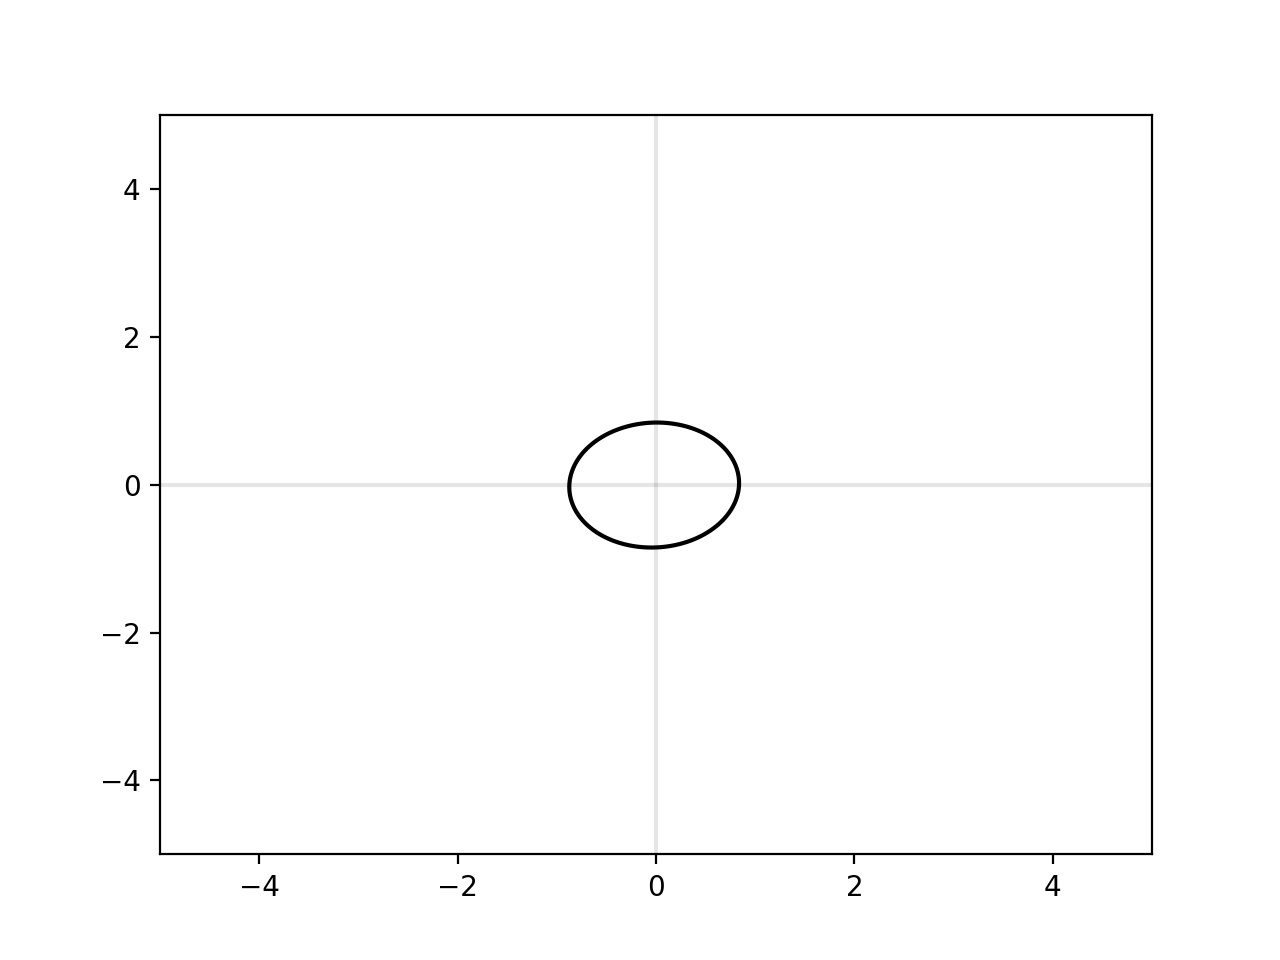
\includegraphics[width=0.7\textwidth]{HW3/part_b_1.jpg}
    \end{minipage}
    \begin{minipage}{0.48\textwidth}
        \centering
        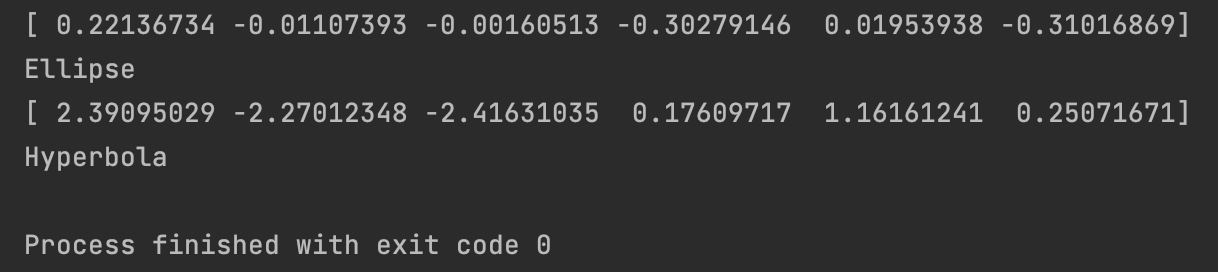
\includegraphics[width=0.7\textwidth]{HW3/outputs_1.jpg}
    \end{minipage}
    \caption{The decision boundary and outputs for part (b); Trial \#1}
    \label{fig:part_b_1}
\end{figure}
\begin{figure}
    \begin{minipage}{0.48\textwidth}
        \centering
        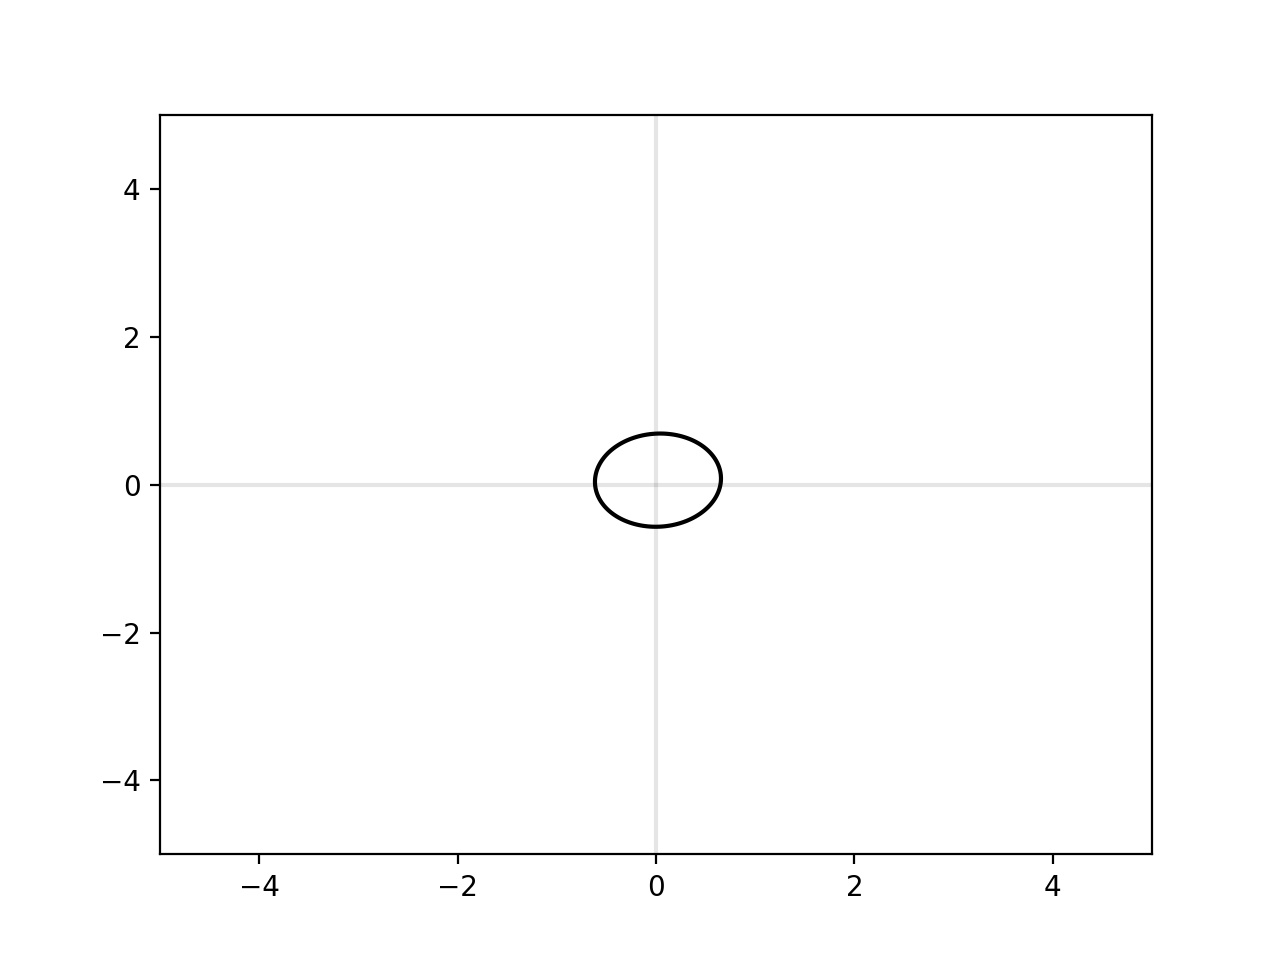
\includegraphics[width=0.7\textwidth]{HW3/part_b_2.jpg}
    \end{minipage}
    \begin{minipage}{0.48\textwidth}
        \centering
        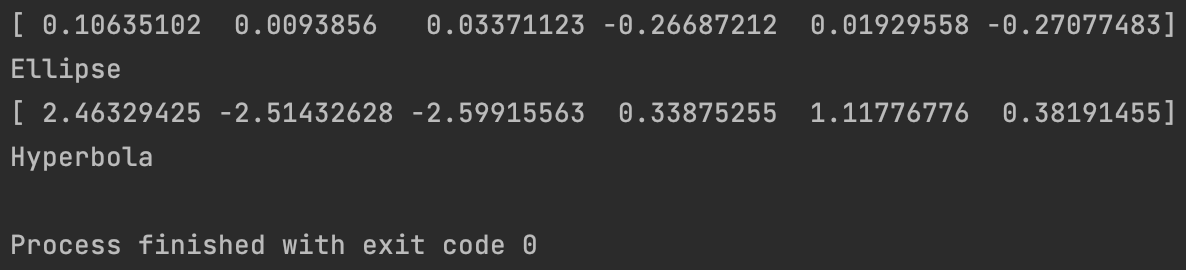
\includegraphics[width=0.7\textwidth]{HW3/outputs_2.jpg}
    \end{minipage}
    \caption{The decision boundary and outputs for part (b); Trial \#2}
    \label{fig:part_b_2}
\end{figure}
\begin{figure}
    \begin{minipage}{0.48\textwidth}
        \centering
        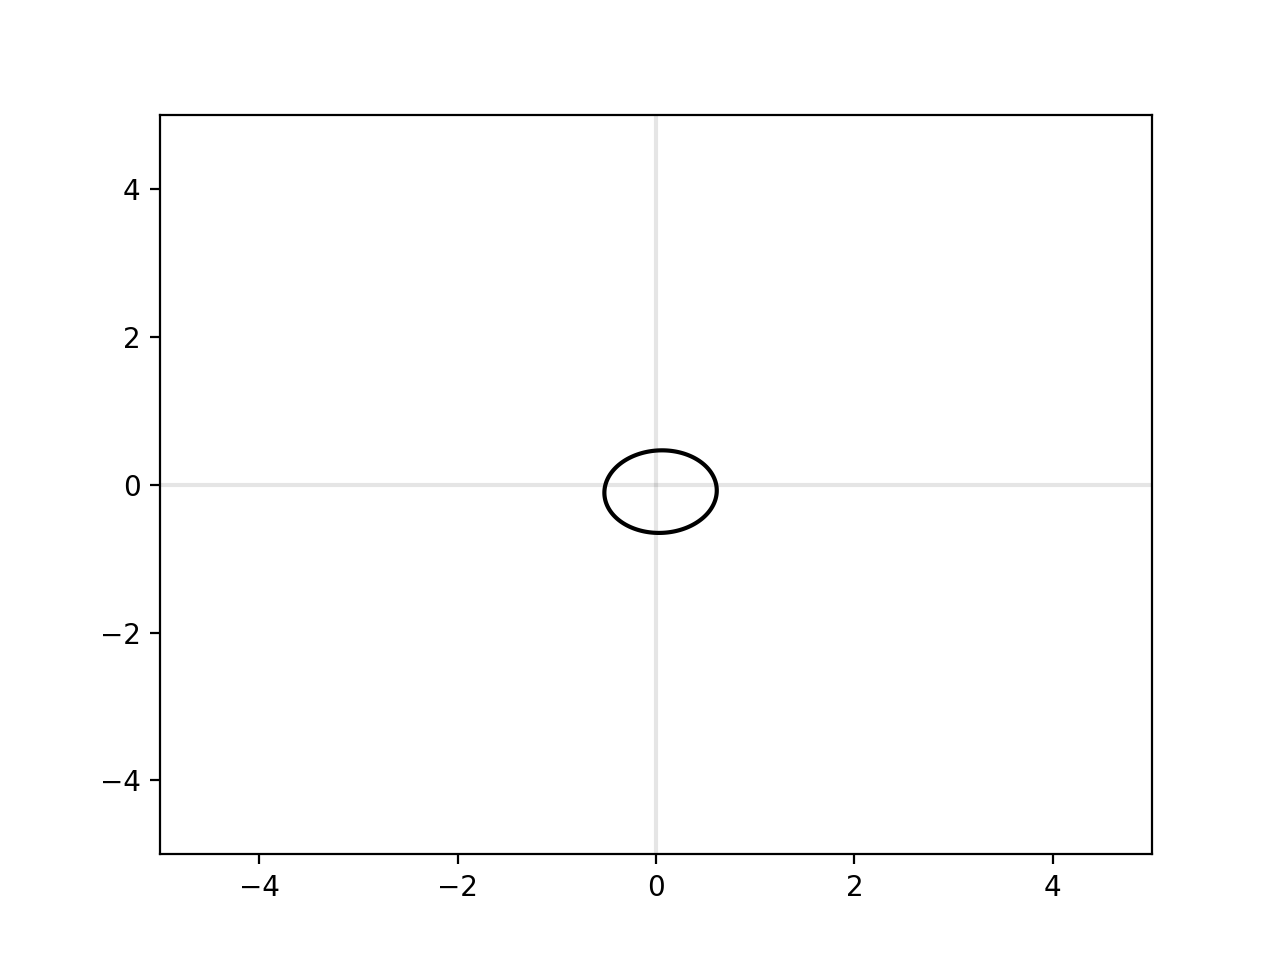
\includegraphics[width=0.7\textwidth]{HW3/part_b_3.jpg}
    \end{minipage}
    \begin{minipage}{0.48\textwidth}
        \centering
        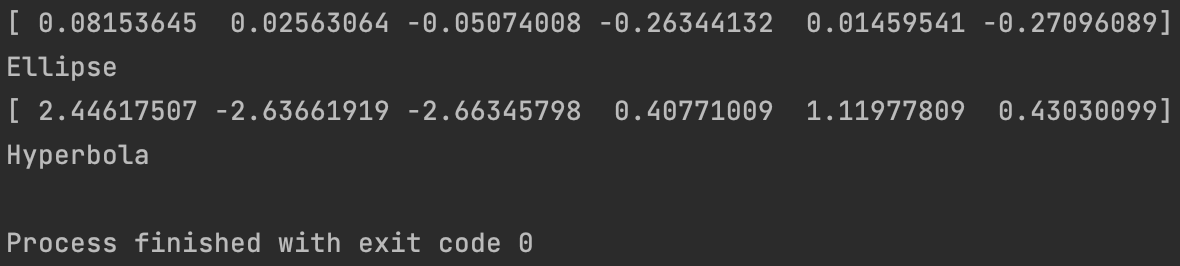
\includegraphics[width=0.7\textwidth]{HW3/outputs_3.jpg}
    \end{minipage}
    \caption{The decision boundary and outputs for part (b); Trial \#3}
    \label{fig:part_b_3}
\end{figure}
\begin{figure}
    \begin{minipage}{0.48\textwidth}
        \centering
        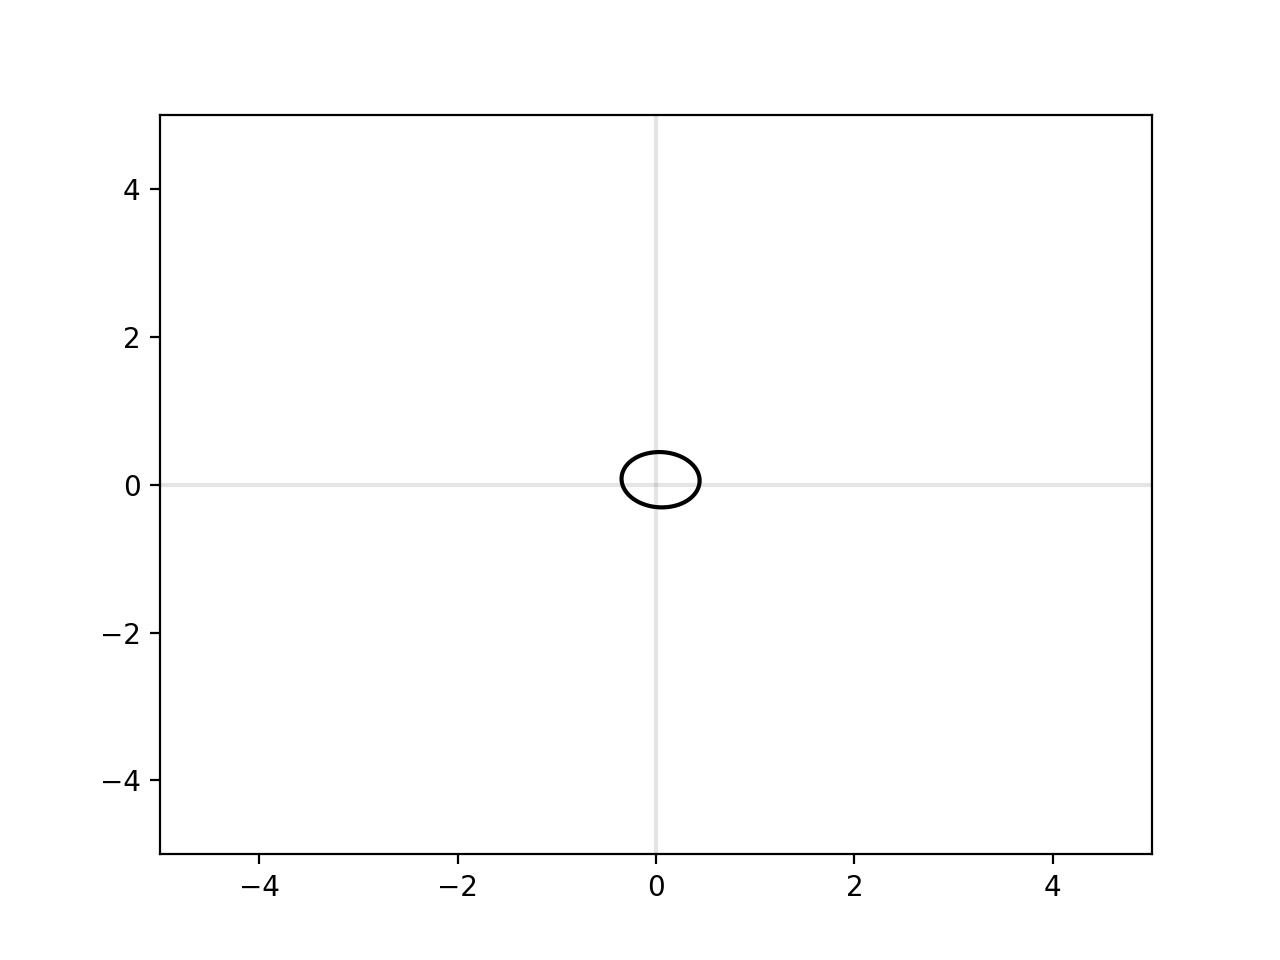
\includegraphics[width=0.7\textwidth]{HW3/part_b_4.jpg}
    \end{minipage}
    \begin{minipage}{0.48\textwidth}
        \centering
        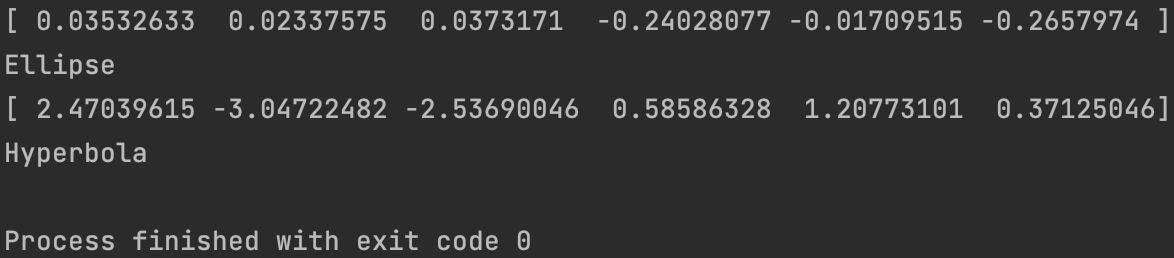
\includegraphics[width=0.7\textwidth]{HW3/outputs_4.jpg}
    \end{minipage}
    \caption{The decision boundary and outputs for part (b); Trial \#4}
    \label{fig:part_b_4}
\end{figure}
\begin{figure}
    \begin{minipage}{0.48\textwidth}
        \centering
        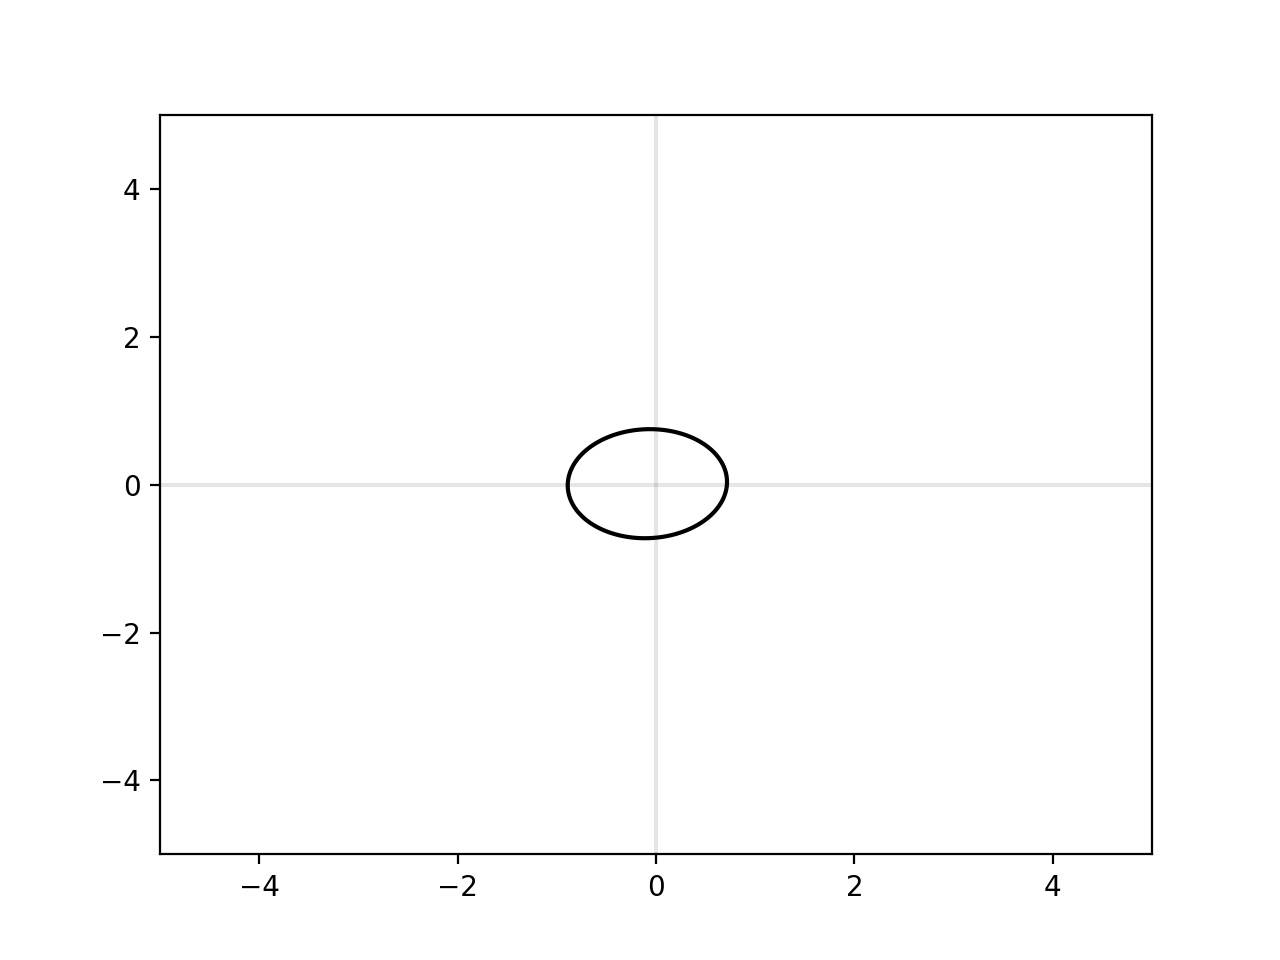
\includegraphics[width=0.7\textwidth]{HW3/part_b_5.jpg}
    \end{minipage}
    \begin{minipage}{0.48\textwidth}
        \centering
        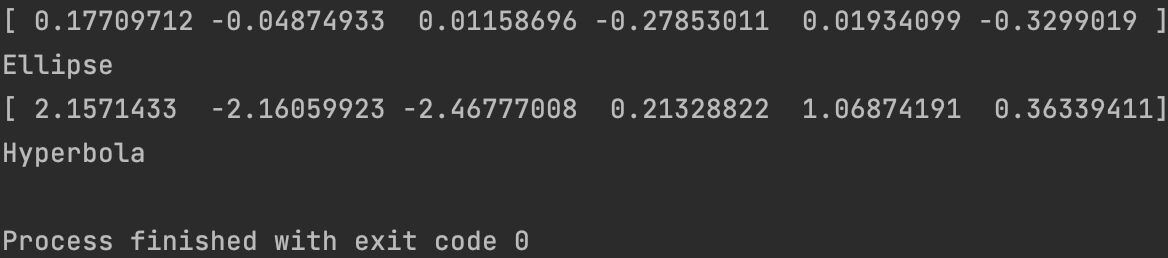
\includegraphics[width=0.7\textwidth]{HW3/outputs_5.jpg}
    \end{minipage}
    \caption{The decision boundary and outputs for part (b); Trial \#5}
    \label{fig:part_b_5}
\end{figure}

\newpage 

\indent As Figure \ref{fig:part_b_1}--\ref{fig:part_b_5} show, we can corroborate that the decision boundary $f(\mathbf{x}) = 0$ of part (b) forms an \emph{ellipse} in $\mathbb{R}^2$ whose center is located nearby the origin $(0, 0)$ via a simple straightforward visualization. Why would the decision boundary $f(\mathbf{x}) = 0$ for part (b) have this shape? One can make a fairly  reasonable guess based on the following intuition: since the optimal polynomial
\begin{equation}
    \label{eqn3}
    f(\mathbf{x}) = f(x_1, x_2) := \theta_{1}^* + \theta_{2}^* x_1 + \theta_{3}^* x_2 + \theta_{4}^* x_{1}^2 + \theta_{5}^* x_1 x_2 + \theta_{6}^* x_{2}^2
\end{equation}
should fit well with the training data $\left\{ \left( \mathbf{x}^{(i)}, y_i \right) : i \in [250] \right\}$, one can anticipate that the decision boundary $f(\mathbf{x}) = 0$ for part (b) closely resembles the boundary of the labeling rule \eqref{eqn1} $\left( = \left\{ (x, y) \in \mathbb{R}^2 : x^2 + y^2 = 1 \right\} \right)$ for part (b) within the region $\left[ -2, 2 \right] \times \left[ -2, 2 \right]$. In this context, we may guess that the decision boundary $f(\mathbf{x}) = 0$ for part (b) would look like an ellipse in $\mathbb{R}^2$ whose center is located nearby the origin $(0, 0)$. \\ [10pt]
\indent (c) The only difference of the part (c) from the part (b) is the sampling scheme of the measurements: we sample $\left\{ \mathbf{x}^{(i)} := \left( x_{1}^{(i)}, x_{2}^{(i)} \right) : i \in [250] \right\}$ uniformly at random from $\left[ 0, 2 \right] \times \left[ 0, 2 \right]$ in lieu of $\left[ -2, 2 \right] \times \left[ -2, 2 \right]$. So the corresponding overall code for part (c) can be summarized as below:

\begin{lstlisting}[language = Python]
import numpy as np
import random
import matplotlib as mpl
import matplotlib.pyplot as plt

def axes():
    plt.axhline(0, alpha=.1)
    plt.axvline(0, alpha=.1)

def label(a, b):     # label a given point in \mathbb{R}^2 according to the rule (4)
    if a**2 + b**2 <= 1:
        return 1
    else:
        return -1

def generate_data_matrix(first_coordinate, second_coordinate):      # construct a proper data matrix (2-dimensional array) of shape length \times 6
    input_length = first_coordinate.shape[0]
    data_matrix = np.zeros((length, 6))
    for i in range(input_length):
        data_matrix[i, 0] = 1
        data_matrix[i, 1] = first_coordinate[i]
        data_matrix[i, 2] = second_coordinate[i]
        data_matrix[i, 3] = first_coordinate[i]**2
        data_matrix[i, 4] = first_coordinate[i]*second_coordinate[i]
        data_matrix[i, 5] = second_coordinate[i]**2
    return data_matrix

def conic_section_discriminant(A, B, C, D, E, F):        # discriminate the conic section Ax^2 + Bxy + Cy^2 + Dx + Ey + F = 0
    discriminant = B**2 - 4*A*C
    if A == C and B == 0:
        return "Circle"
    elif discriminant < 0:
        return "Ellipse"
    elif discriminant == 0:
        return "Parabola"
    else:
        return "Hyperbola"

length = 250     # number of samples
first_coordinate_2 = np.dot(2, np.random.rand(length))     # the first coordinates of 250 samples chosen uniformly at random from [0, 2] \times [0, 2]
second_coordinate_2 = np.dot(2, np.random.rand(length))    # the second coordinates of 250 samples chosen uniformly at random from [0, 2] \times [0, 2]
y_2 = np.zeros(length)     # initialize vector of labels for part (c)
num_2 = 0
for i in range(length):
    y_2[i] = label(first_coordinate_2[i], second_coordinate_2[i])     # label the 250 random sample points according to the rule (4)
    if y_2[i] > 0:
        num_2 = num_2 + 1

A_2 = generate_data_matrix(first_coordinate_2, second_coordinate_2)
theta_2 = my_lstsq(A_2, y_2)     # compute the optimal order-2 polynomial that minimizes (3)
print(theta_2)
print(conic_section_discriminant(theta_2[3], theta_2[4], theta_2[5], theta_2[1], theta_2[2], theta_2[0]))     # discriminate the conic section formed as the zero set of the optimal order-2 polynomial that minimizes (3) (= the decision boundary)

x = np.linspace(-5, 5, 4000)
y = np.linspace(-5, 5, 4000)
x, y = np.meshgrid(x, y)
axes()
plt.contour(x, y, (theta_2[3]*x**2 + theta_2[4]*x*y + theta_2[5]*y**2 + theta_2[1]*x + theta_2[2]*y + theta_2[0]), [0], colors='k')
plt.show()
\end{lstlisting}

\indent Moreover, the corresponding numerical simulation results are obtained as follows over 5 trials, which were also conducted in the demonstration of Figure \ref{fig:part_b_1}--\ref{fig:part_b_5}:
\begin{figure}
    \begin{minipage}{0.48\textwidth}
        \centering
        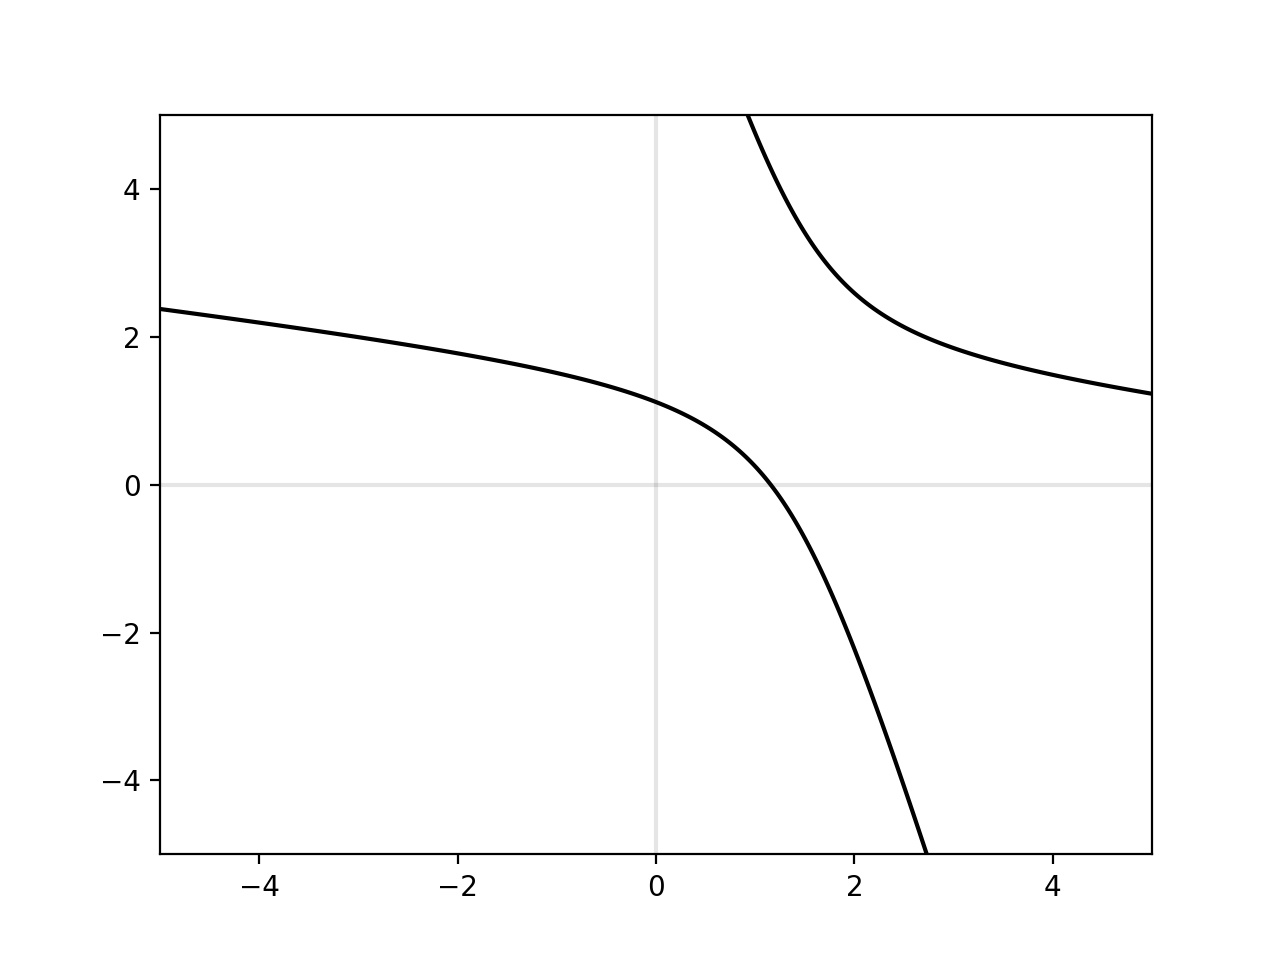
\includegraphics[width=0.7\textwidth]{HW3/part_c_1.jpg}
    \end{minipage}
    \begin{minipage}{0.48\textwidth}
        \centering
        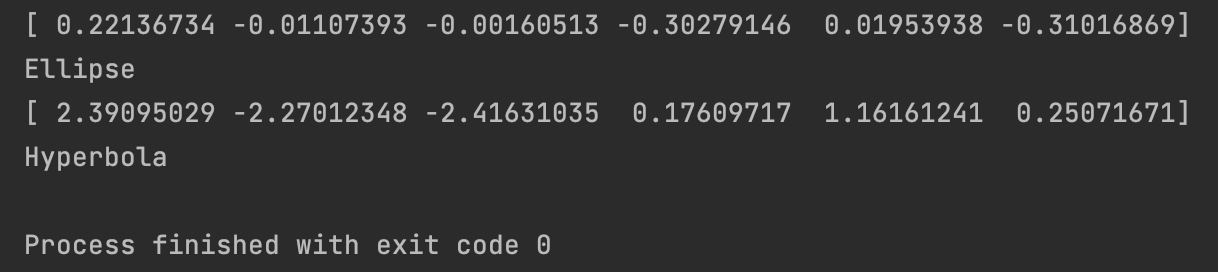
\includegraphics[width=0.7\textwidth]{HW3/outputs_1.jpg}
    \end{minipage}
    \caption{The decision boundary and outputs for part (c); Trial \#1}
    \label{fig:part_c_1}
\end{figure}
\begin{figure}
    \begin{minipage}{0.48\textwidth}
        \centering
        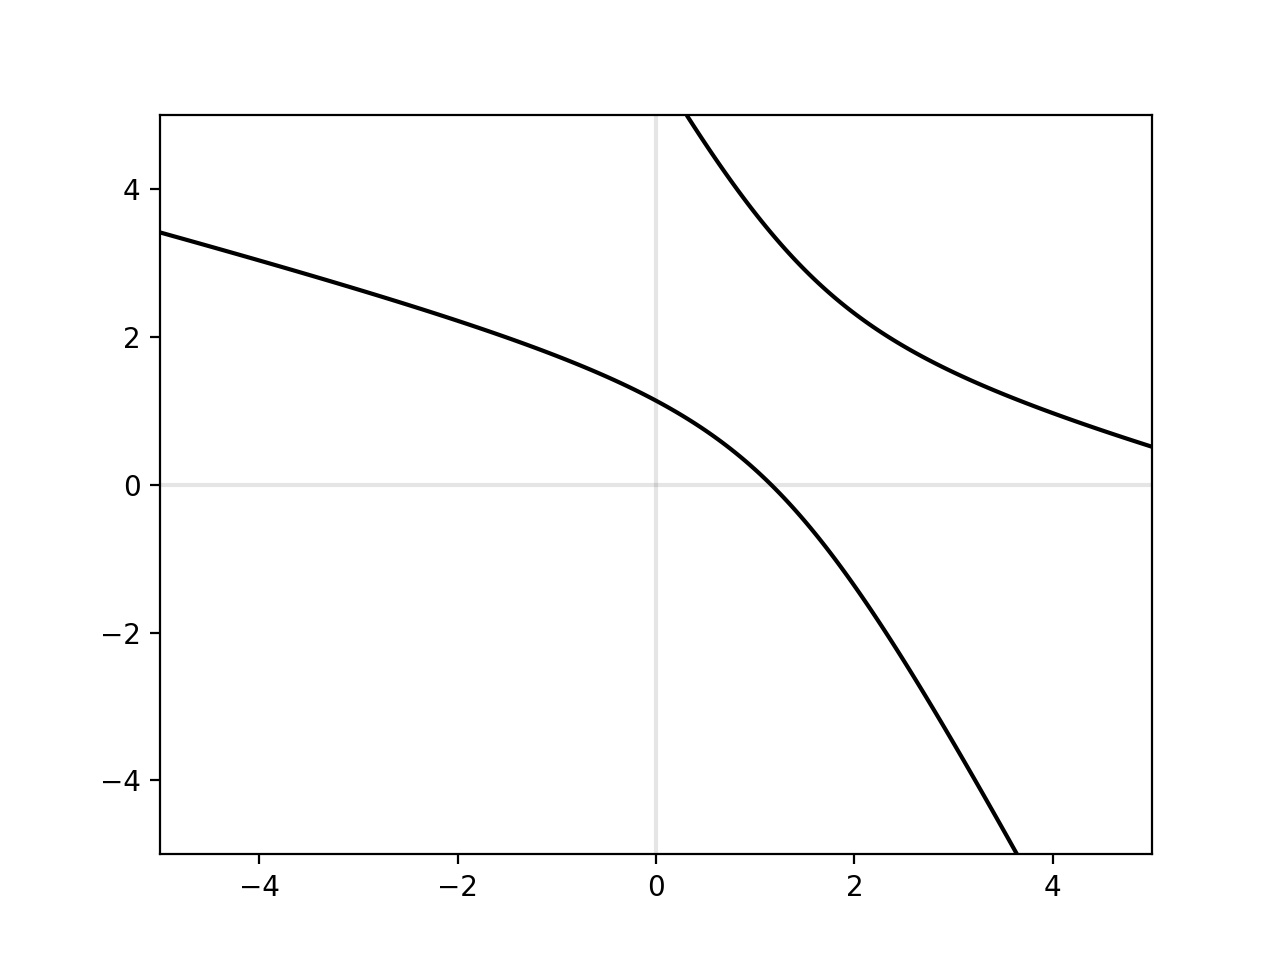
\includegraphics[width=0.7\textwidth]{HW3/part_c_2.jpg}
    \end{minipage}
    \begin{minipage}{0.48\textwidth}
        \centering
        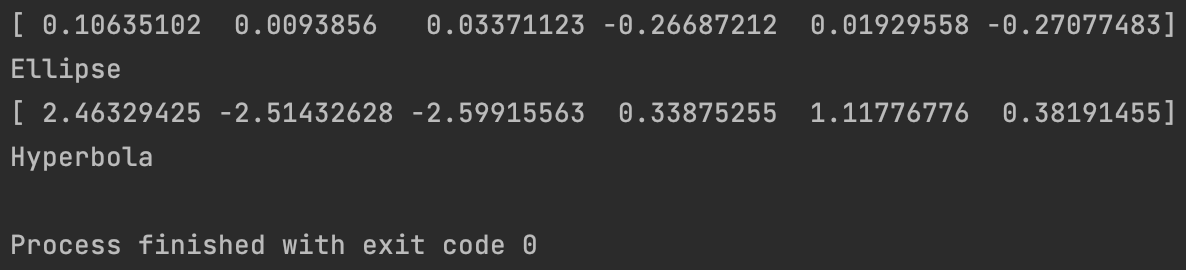
\includegraphics[width=0.7\textwidth]{HW3/outputs_2.jpg}
    \end{minipage}
    \caption{The decision boundary and outputs for part (c); Trial \#2}
    \label{fig:part_c_2}
\end{figure}
\begin{figure}
    \begin{minipage}{0.48\textwidth}
        \centering
        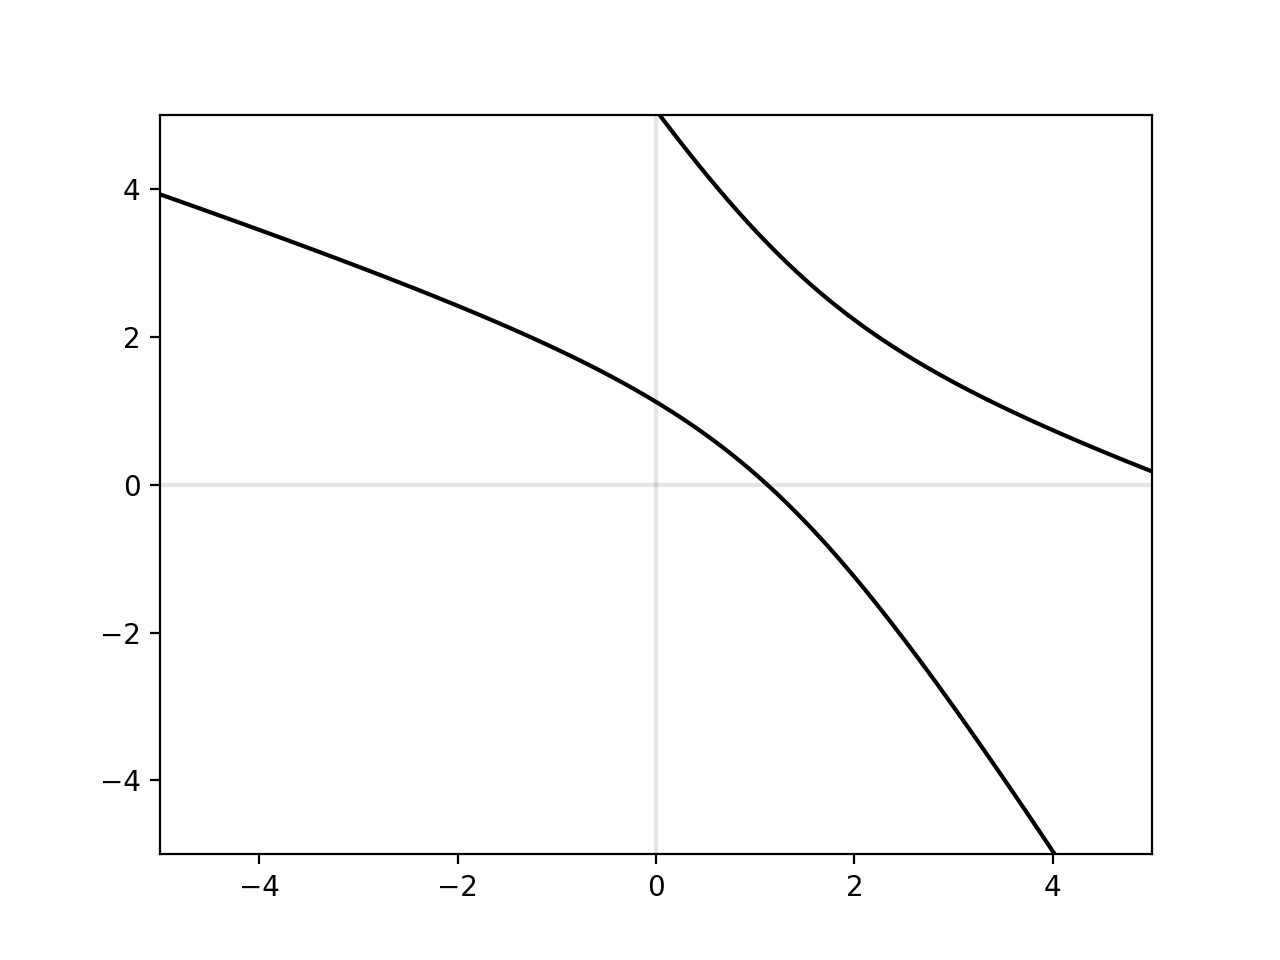
\includegraphics[width=0.7\textwidth]{HW3/part_c_3.jpg}
    \end{minipage}
    \begin{minipage}{0.48\textwidth}
        \centering
        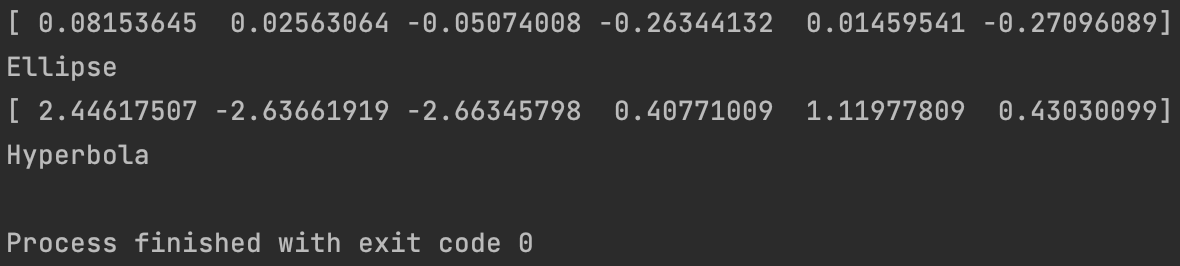
\includegraphics[width=0.7\textwidth]{HW3/outputs_3.jpg}
    \end{minipage}
    \caption{The decision boundary and outputs for part (c); Trial \#3}
    \label{fig:part_c_3}
\end{figure}
\begin{figure}
    \begin{minipage}{0.48\textwidth}
        \centering
        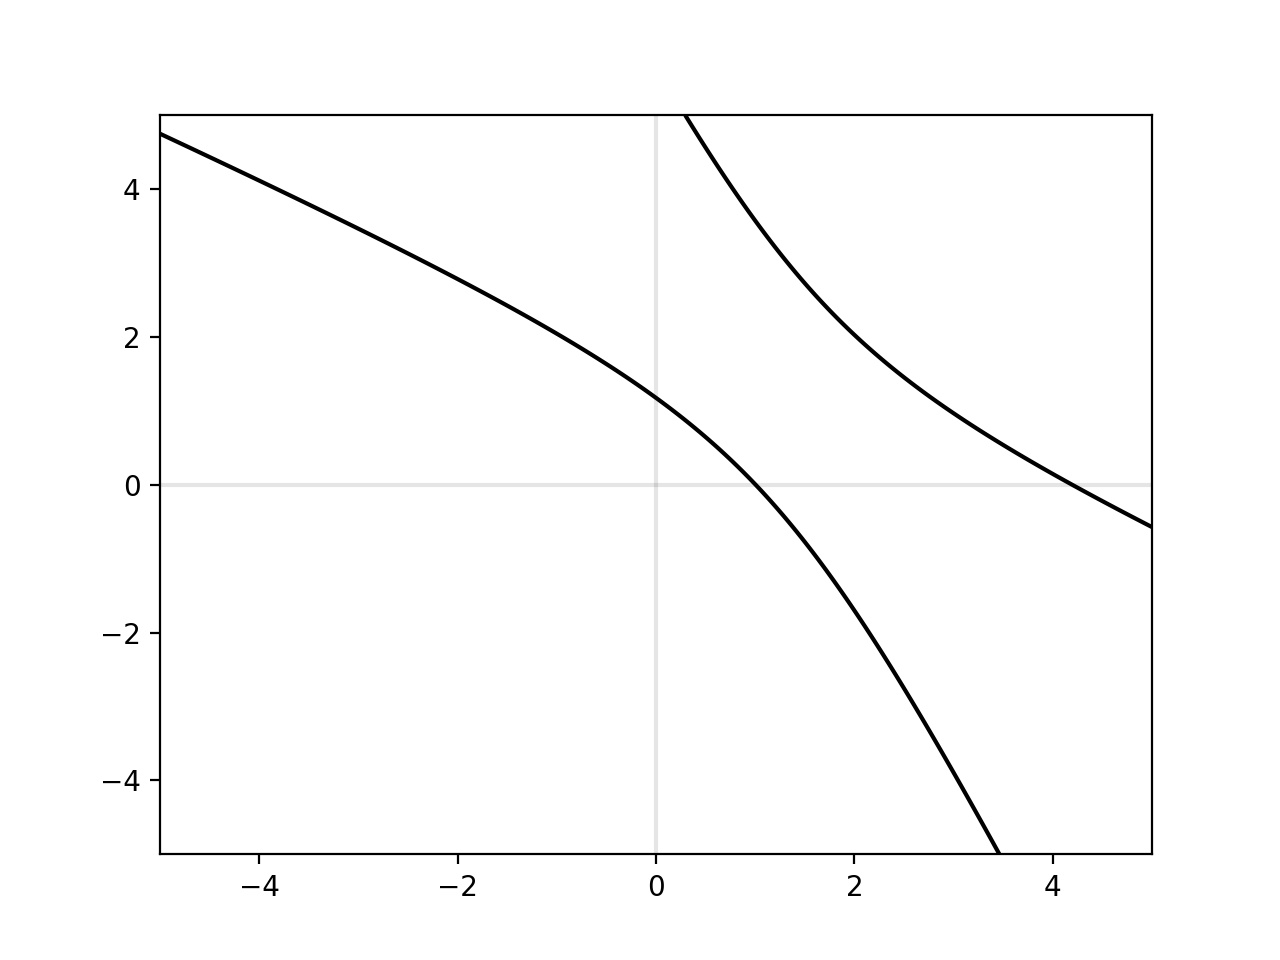
\includegraphics[width=0.7\textwidth]{HW3/part_c_4.jpg}
    \end{minipage}
    \begin{minipage}{0.48\textwidth}
        \centering
        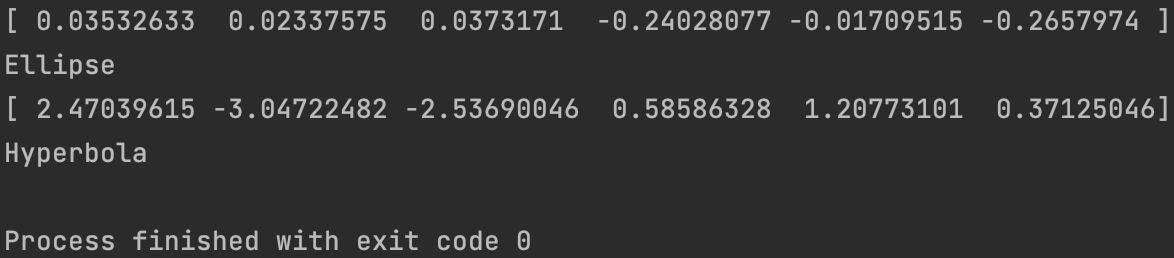
\includegraphics[width=0.7\textwidth]{HW3/outputs_4.jpg}
    \end{minipage}
    \caption{The decision boundary and outputs for part (c); Trial \#4}
    \label{fig:part_c_4}
\end{figure}
\begin{figure}
    \begin{minipage}{0.48\textwidth}
        \centering
        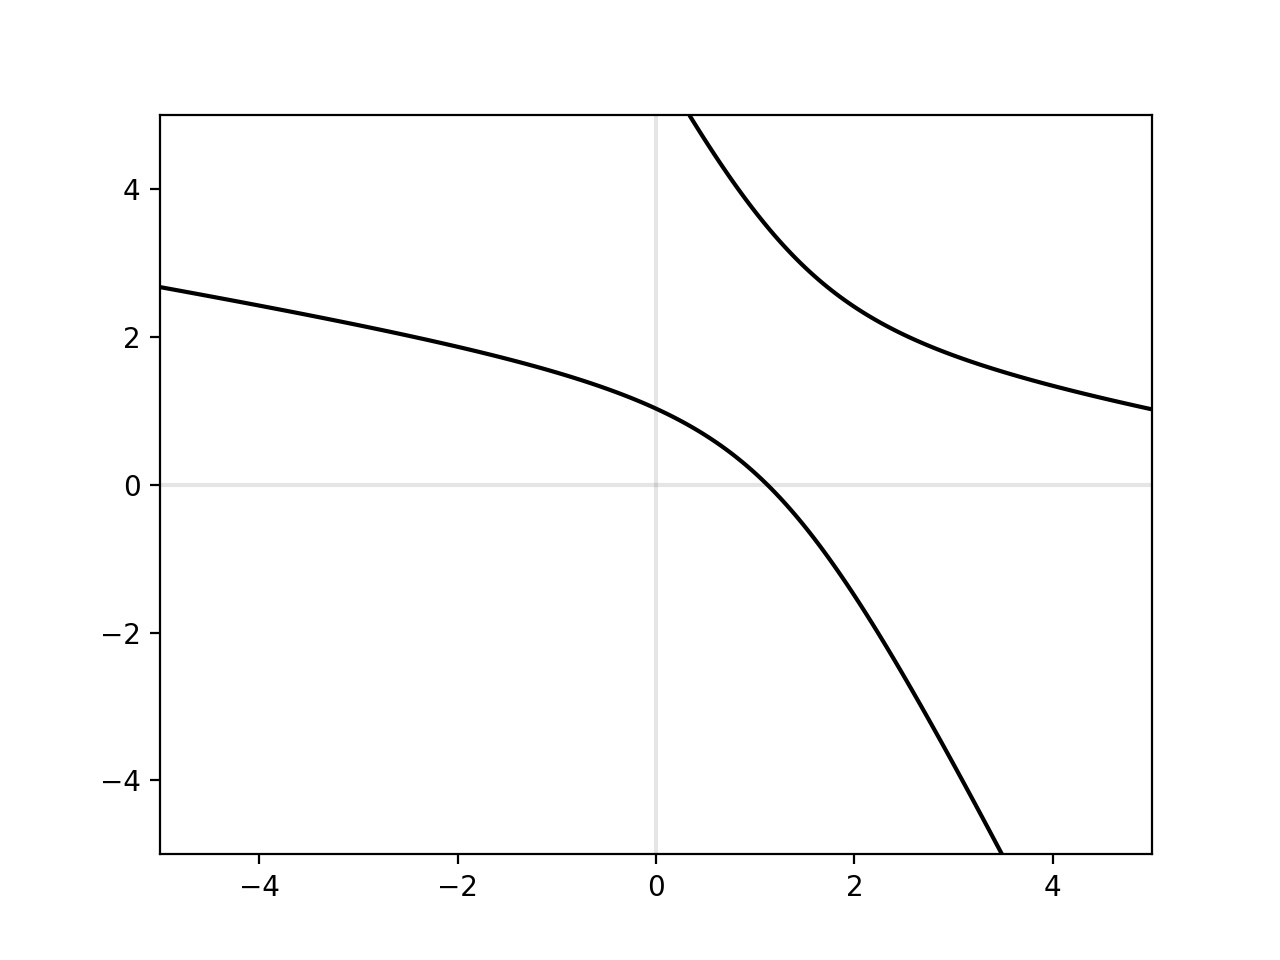
\includegraphics[width=0.7\textwidth]{HW3/part_c_5.jpg}
    \end{minipage}
    \begin{minipage}{0.48\textwidth}
        \centering
        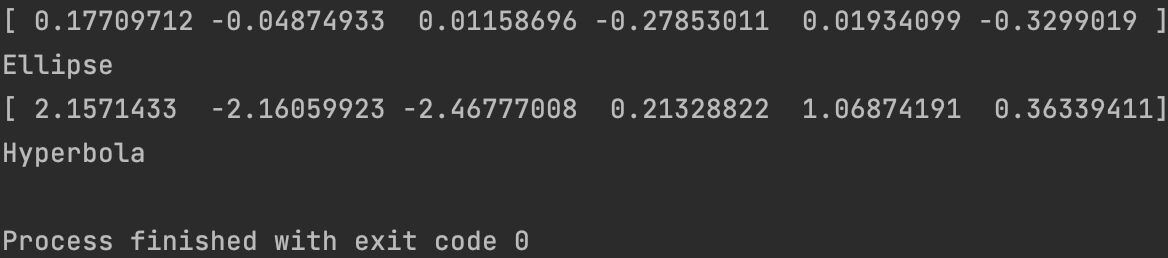
\includegraphics[width=0.7\textwidth]{HW3/outputs_5.jpg}
    \end{minipage}
    \caption{The decision boundary and outputs for part (c); Trial \#5}
    \label{fig:part_c_5}
\end{figure}

\newpage

\indent  As Figure \ref{fig:part_c_1}--\ref{fig:part_c_5} demonstrate, one may empirically confirm that the decision boundary $f(\mathbf{x}) = 0$ of part (c) forms a \emph{hyperbola} in $\mathbb{R}^2$. At this point, as part (b), one can make a guess of the shape of the decision boundary $f(\mathbf{x}) = 0$ for part (c) with the aid of an analogous intuition: since the optimal polynomial \eqref{eqn3} should fit well with the training examples $\left\{ \left( \mathbf{x}^{(i)}, y_i \right) : i \in [250] \right\}$, we may expect that the decision boundary $f(\mathbf{x}) = 0$ for part (c) looks similar with the boundary of the labeling rule \eqref{eqn1} $\left( = \left\{ (x, y) \in \mathbb{R}^2 : x, y \geq 0 \ \& \ x^2 + y^2 = 1 \right\} \right)$ for part (c) within the region $\left[ 0, 2 \right] \times \left[ 0, 2 \right]$. It is worth to notice that the decision boundary $f(\mathbf{x}) = 0$ for part (c) has no need for being akin to the remaining parts of the unit circle in $\mathbb{R}^2$. Indeed, we can find that the intersections of the hyperbolas in Figure \ref{fig:part_c_1}--\ref{fig:part_c_5} and the rectangular region $\left[ 0, 2 \right] \times \left[ 0, 2 \right]$ look very similar to the first quadrant part of the unit circle $\left( = \left\{ (x, y) \in \mathbb{R}^2 : x, y \geq 0 \ \& \ x^2 + y^2 = 1 \right\} \right)$. So one can argue that the empirical results in Figure \ref{fig:part_c_1}--\ref{fig:part_c_5} match fairly well with our intuition. However, in my opinion, it would be difficult to determine the exact shape of the conic section $f(\mathbf{x}) = 0$ for part (c), which is determined by its discriminant (or its eccentricity), solely based on such intuitions.

\newpage

\appendix


\bibliographystyle{plain}
\bibliography{main.bib}

\end{document}